\chapter{SysML, ERTMSFormalSpecs and Eclipse/Polarsys}
\label{sec:sysML-EFS}

The proposed approach combines three tools existing today to provide an integrated toolchain, from system design 
to code generation.

\begin{figure}[b!]
	\centering
		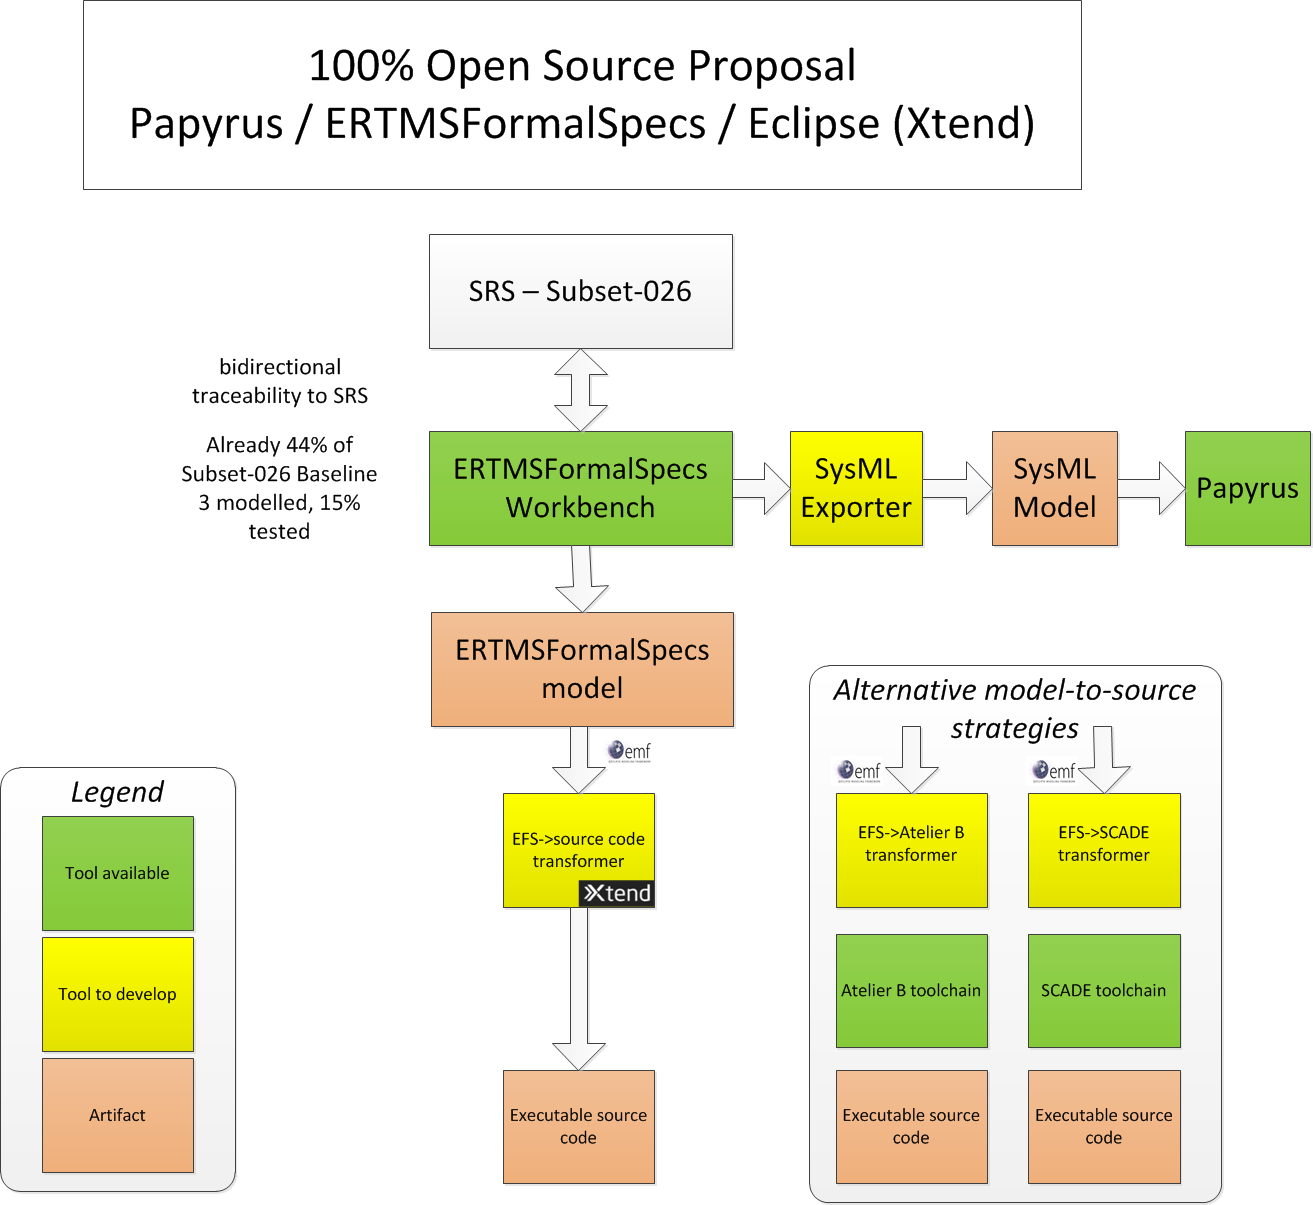
\includegraphics[width=\textwidth]{images/ERTMSFormalSpecsProposal_V2.png}
		\caption{SysML, ErtmsFormalSpec and Eclipse/Polarsys Proposal}
	\label{fig:ERTMSFormalSpecsProposal}
\end{figure}

\section{Description of the approach for OpenETCS design process}

The proposed toolchain is illustrated in Figure \ref{fig:ERTMSFormalSpecsProposal}.

The blue boxes of the overall design process are covered in the following manner:

SRS box: Using Papyrus for visualizing the high-level ERTMSFormalSpecs model design in SysML language. 

Sub-system semi-formal model box: Using ERTMSFormalSpecs to model the complete SRS into a semi-formal model.

Software semi-formal model + architecture description box: Shall be done inside the ERTMSFormalSpecs->source transformer box, using XText Eclipse framework.
The ERTMSFormalSpecs->source transformer shall transform the ERTMSFormalSpecs model into target source code. The architecture and software model of generated source code is part of the ERTMSFormalSpecs->source transformer. The actual target language shall be chosen in agreement with WP5 (demonstrator).

Target source code box: This box is covered by the source code generated by the ERTMSFormalSpecs->source transformer. This source code can then be compiled and executed on the demonstrator hardware.

Note: The ERTMSFormalSpecs->source transformer is not available today, and shall have to be implemented in the scope of the OpenETCS project. This is detailed in further Shortcomings and Ongoing work sections.

Note: the ERTMSFormalSpecs->source transformer doesn't neet to be qualified according to CENELEC standards, to fullfill the two following objectives of the OpenETCS project, i.e. 1/ a complete Subset-026 semi-formal model and 2/ generated, non-vital source code running on demonstrator platform (See Section 3. OPENETCS PROJECT – SCOPE OF WORK AND OBJECTIVES in \citep{WP3_WP4_WP7_SafetyMeetingMinutes_April2013})

\section{Integration of the approach with SysML/Papyrus}

The proposed approach uses SysML/Papyrus as a visualization tool on the ERTMSFormalSpecs model. A SysML exporter component (yet to be developed) shall transform selected part of the ERTMSFormalSpecs model into SysML artifacts (state machines, interaction diagrams, module diagrams, data flows, etc) in order to improve readability of the ERTMSFormalSpecs model thanks to SysML. 

In a second phase, if changes are brought to the SysML model, the SysML exporter component could be extended in order to provide round-trip engineering between the ERTMSFormalSpecs model and the generated SysML model, so that changes brought to the SysML model are propagated to the ERTMSFormalSpecs model.

Some questions are open:

- What is the optimal mapping between ERTMSFormalSpecs model elements and SysML diagrams and elements, in order to maximize model readability and verifiability? 
- How can round-trip engineering be implemented, to propagate changes brought to the SysML model back to the original ERTMSFormalSpecs model?

\section{Integration of the approach with Eclipse}

SysML/Papyrus is completely based on Eclipse.

ERTMSFormalSpecs supports today an EMF interface, enabling Eclipse-based tools to reuse the existing ERTMSFormalSpecs model.

Technically, ERTMSFormalSpecs is implemented mostly in C\# and .Net (the ERTMSFormalSpecs workbench) and also has a java-based component, capable of exporting the ERTMSFormalSpecs xml model into an EMF store, so that the ERTMSFormalSpecs model can be accessed from the Eclipse world. 

Eclipse/Polarsys tools are also based on Eclipse, raising no integration concerns.

\section{Benefits versus OpenETCS requirements}

The benefits of the SysML/Papyrus/ERTMSFormalSpecs/Eclipse proposal are the following:

\begin{itemize}
	\item As of today, already 44\% of Subset-026 requirements modelled. This proposal enables the OpenETCS project to start with a headstart, instead of nothing.
	\item ERTMSFormalSpecs is the only semi-formal candidate to have built-in braking curves modellings and visualization, verified with the ERA model
	\item ERTMSFormalSpecs has very strong support for traceability to the Subset-026, and to the Subset-076 for test cases. More specifically, inside the ERTMSFormalSpecs workbench, every requirements of Subset-026 can be linked to one or more model artifacts. These links are used by the ERTMSFormalSpecs workbench to generate specification coverage reports. Tests from Subset-076 can also be linked to requirements of Subset-026. For more details, see the online ERTMSFormalSpecs User Guide.  
	\item ERTMSFormalSpecs has its domain-specific language, which is highly productive to model Subset-026, thanks to its expressivity, illustrated by the primitives
developed for braking curves and scalable, as is demonstrated by the large fraction of the Subset-026 which has been modelled so far
	\item Fully open-source (ERTMSFormalSpecs under EUPL license, others open source). Note: the alternative model-to-source strategies (using Atelier B or SCADE)  might not be fully open-source. 
	\item ERTMSFormalSpecs model can be transformed automatically to SCADE model (confirmed by ESTEREL Technologies in Munich meeting), allowing to choose SCADE as a code generation backend in case Eclipse/Polarsys would not meet the project requirements
	\item The three elements of the toolchain (Papyrus, ERTMSFormalSpecs and Eclipse) boast an active community of users and are supported by open-source business cases
\end{itemize}

\section{Shortcommings versus OpenETCS requirements}

The shortcomings of the SysML/Papyrus/ERTMSFormalSpecs/Eclipse proposal are the following:

\begin{itemize}
	\item ERTMSFormalSpecs has a perfectible look and feel and lacks graphical rendering of the architecture. \emph{This shortcoming might be addressed with the integration of SysML as a visualization language.}
	\item As of today, the code generation in Eclipse, transforming the ERTMSFormalSpecs in generated source code, is not yet available, and must be developed during task 3.8 of the project. This should be a relatively easy task, as the code generator doesn't need to be qualified according to CENELEC standards (See Section 3. OPENETCS PROJECT – SCOPE OF WORK AND OBJECTIVES in \citep{WP3_WP4_WP7_SafetyMeetingMinutes_April2013}). \emph{This shortcoming can be mitigated by integrating the scade code generator as an alternate solution, or by transforming the ERTMSFormalSpecs model to Atelier B model, to enjoy Atelier B's readily available code generators.}
\end{itemize}

\section{On going work for openETCS project}

The following elements should be further developed during the OpenETCS project, to alleviate the shortcomings listed above:

\begin{enumerate}
  \item Develop conceptual and technical strategies to integrate SysML with ERTMSFormalSpecs model, going beyond the state-of-the-art. The state-of-the-art in integrating SysML models and industrial (semi-)formal languages being SCADE System, in which only the module, interfaces and dataflows are connected to the lower-level model.
	\item Further develop ERTMSFormalSpecs model to cover 100\% of Subset-026, 100\% of Subset-076, and to fully test the model within ERTMSFormalSpecs. 
	\item Either implement a full eclipse-based version of the ERTMSFormalSpecs workbench for model development, traceability and testing, or improve the ERTMSFormalSpecs user interface to be fully productive for T3.5 and T3.6 tasks
	\item Develop code-generation strategies during T3.8 tasks
\end{enumerate}

Among theses tasks, Task 2 and 4 fit inside the WP3 existing tasks, and do not need additional skills than the ones present in the OpenETCS consortium as of today. Task 1 is also seriously represented in the consortium, in which a lot of SysML experience is present. 

Task 3 (porting the ERTMSFormalSpecs workbench to Eclipse) is a task that falls in the scope of WP7, and for which Eclipse development and integration skills are required.

\section{Conclusion and other comments}

As a conclusion, the SysML/Papyrus/ERTMSFormalSpecs/Eclipse proposal has as 3 key strengths 1/ to be fully available today for the WP3 modelling tasks, which are the most urgent 2/ to already model 44\% of Subset-026, and 3/ to be fully open-source. 

Moreover, it proposes a realistic technical foundation to achieve the WP3 and projects top-priority objectives with the skills and resources available in the project.
